%===============================================================================
% LaTeX sjabloon voor de bachelorproef toegepaste informatica aan HOGENT
% Meer info op https://github.com/HoGentTIN/latex-hogent-report
%===============================================================================

\documentclass[dutch,dit,thesis]{hogentreport}

% TODO:
% - If necessary, replace the option `dit`' with your own department!
%   Valid entries are dbo, dbt, dgz, dit, dlo, dog, dsa, soa
% - If you write your thesis in English (remark: only possible after getting
%   explicit approval!), remove the option "dutch," or replace with "english".

\usepackage{lipsum} % For blind text, can be removed after adding actual content

%% Pictures to include in the text can be put in the graphics/ folder
\graphicspath{{graphics/}}

%% For source code highlighting, requires pygments to be installed
%% Compile with the -shell-escape flag!
\usepackage[section]{minted}
%% If you compile with the make_thesis.{bat,sh} script, use the following
%% import instead:
%% \usepackage[section,outputdir=../output]{minted}
\usemintedstyle{solarized-light}
\definecolor{bg}{RGB}{253,246,227} %% Set the background color of the codeframe

%% Change this line to edit the line numbering style:
\renewcommand{\theFancyVerbLine}{\ttfamily\scriptsize\arabic{FancyVerbLine}}

%% Macro definition to load external java source files with \javacode{filename}:
\newmintedfile[javacode]{java}{
    bgcolor=bg,
    fontfamily=tt,
    linenos=true,
    numberblanklines=true,
    numbersep=5pt,
    gobble=0,
    framesep=2mm,
    funcnamehighlighting=true,
    tabsize=4,
    obeytabs=false,
    breaklines=true,
    mathescape=false
    samepage=false,
    showspaces=false,
    showtabs =false,
    texcl=false,
}

% Other packages not already included can be imported here

%%---------- Document metadata -------------------------------------------------
% TODO: Replace this with your own information
\author{Berton Jasper}
\supervisor{Dhr. S. Verschraege}
\cosupervisor{Dhr. J. Buysse}
\title
    {Hoe kan het ontwikkelen van een interne applicatie het handmatig testen van een privaat netwerk vereenvoudigen?}
\academicyear{\advance\year by -1 \the\year--\advance\year by 1 \the\year}
\examperiod{2}
\degreesought{\IfLanguageName{dutch}{Professionele bachelor in de toegepaste informatica}{Bachelor of applied computer science}}
\partialthesis{false} %% To display 'in partial fulfilment'
%\institution{Internshipcompany BVBA.}

%% Add global exceptions to the hyphenation here
\hyphenation{back-slash}

%% The bibliography (style and settings are  found in hogentthesis.cls)
\addbibresource{bachproef.bib}            %% Bibliography file
\addbibresource{../voorstel/voorstel.bib} %% Bibliography research proposal
\defbibheading{bibempty}{}

%% Prevent empty pages for right-handed chapter starts in twoside mode
\renewcommand{\cleardoublepage}{\clearpage}

\renewcommand{\arraystretch}{1.2}

%% Content starts here.
\begin{document}

%---------- Front matter -------------------------------------------------------

\frontmatter

\hypersetup{pageanchor=false} %% Disable page numbering references
%% Render a Dutch outer title page if the main language is English
\IfLanguageName{english}{%
    %% If necessary, information can be changed here
    \degreesought{Professionele Bachelor toegepaste informatica}%
    \begin{otherlanguage}{dutch}%
       \maketitle%
    \end{otherlanguage}%
}{}

%% Generates title page content
\maketitle
\hypersetup{pageanchor=true}

%%=============================================================================
%% Voorwoord
%%=============================================================================

\chapter*{\IfLanguageName{dutch}{Woord vooraf}{Preface}}%
\label{ch:voorwoord}

%% TODO:
%% Het voorwoord is het enige deel van de bachelorproef waar je vanuit je
%% eigen standpunt (``ik-vorm'') mag schrijven. Je kan hier bv. motiveren
%% waarom jij het onderwerp wil bespreken.
%% Vergeet ook niet te bedanken wie je geholpen/gesteund/... heeft

\lipsum[1-2]
%%=============================================================================
%% Samenvatting
%%=============================================================================

% TODO: De "abstract" of samenvatting is een kernachtige (~ 1 blz. voor een
% thesis) synthese van het document.
%
% Een goede abstract biedt een kernachtig antwoord op volgende vragen:
%
% 1. Waarover gaat de bachelorproef?
% 2. Waarom heb je er over geschreven?
% 3. Hoe heb je het onderzoek uitgevoerd?
% 4. Wat waren de resultaten? Wat blijkt uit je onderzoek?
% 5. Wat betekenen je resultaten? Wat is de relevantie voor het werkveld?
%
% Daarom bestaat een abstract uit volgende componenten:
%
% - inleiding + kaderen thema
% - probleemstelling
% - (centrale) onderzoeksvraag
% - onderzoeksdoelstelling
% - methodologie
% - resultaten (beperk tot de belangrijkste, relevant voor de onderzoeksvraag)
% - conclusies, aanbevelingen, beperkingen
%
% LET OP! Een samenvatting is GEEN voorwoord!

%%---------- Nederlandse samenvatting -----------------------------------------
%
%%---------- Samenvatting -----------------------------------------------------
% De samenvatting in de hoofdtaal van het document

\chapter*{\IfLanguageName{dutch}{Samenvatting}{Abstract}}




%---------- Inhoud, lijst figuren, ... -----------------------------------------

\tableofcontents

% In a list of figures, the complete caption will be included. To prevent this,
% ALWAYS add a short description in the caption!
%
%  \caption[short description]{elaborate description}
%
% If you do, only the short description will be used in the list of figures

\listoffigures

% If you included tables and/or source code listings, uncomment the appropriate
% lines.
%\listoftables
%\listoflistings

% Als je een lijst van afkortingen of termen wil toevoegen, dan hoort die
% hier thuis. Gebruik bijvoorbeeld de ``glossaries'' package.
% https://www.overleaf.com/learn/latex/Glossaries

%---------- Kern ---------------------------------------------------------------

\mainmatter{}

% De eerste hoofdstukken van een bachelorproef zijn meestal een inleiding op
% het onderwerp, literatuurstudie en verantwoording methodologie.
% Aarzel niet om een meer beschrijvende titel aan deze hoofdstukken te geven of
% om bijvoorbeeld de inleiding en/of stand van zaken over meerdere hoofdstukken
% te verspreiden!

%%=============================================================================
%% Inleiding
%%=============================================================================

\chapter{\IfLanguageName{dutch}{Inleiding}{Introduction}}%
\label{ch:inleiding}

Doorheen de afgelopen decennia is de mens steeds afhankelijker geworden van een zeker apparaat, namelijk de gsm. Er zijn al applicaties die ons het leven gemakkelijker maken maar ze leggen wel een ander pijnpunt bloot , namelijk de nood om continu verbonden zijn met het wereldwijde web. De kracht van openbare netwerken en Wifi installaties groeien met de dag maar in verscheidene situaties is er nog steeds nood voor extra ondersteuning zodat in bepaalde omstandigheden indien het nodig is iemand niet zonder een verbinding valt. \\
Een privaat netwerk kan een oplossing bieden om te zorgen dat noodzakelijke technologie blijft draaien. Hierbij kan de consument zelf beslissen wie er toegang heeft tot de infrastructuur om zo tegen te gaan dat er een overbelasting plaatsvind. Men mag dit wel niet verwarren met een Wifi netwerk dat via een wachtwoord is beveiligd want de data transporteert zich via een spectrum van binnen een cellulair netwerk. Doordat de aanbieder eigenaar is van dit spectrum is deze bandbreedte volledig vrij voor de consument. Een nadeel dat hierbij opkomt is dat men dan wel verwacht dat deze opstelling te alle tijde in werking blijft. Men kan dan namelijk wel de vraag stellen of er netwerken genoeg zijn om specifieke test applicaties te verantwoorden. Volgens \textcite{Dux2023}  was er een marktpotentieel van 1212 bedrijven met toepassingen van een privaat netwerk aanwezig. 
\section{\IfLanguageName{dutch}{Probleemstelling}{Problem Statement}}%
\label{sec:probleemstelling}

%%%Uit je probleemstelling moet duidelijk zijn dat je onderzoek een meerwaarde heeft voor een concrete doelgroep. De doelgroep moet goed gedefinieerd en afgelijnd zijn. Doelgroepen als ``bedrijven,'' ``KMO's'', systeembeheerders, enz.~zijn nog te vaag. Als je een lijstje kan maken van de personen/organisaties die een meerwaarde zullen vinden in deze bachelorproef (dit is eigenlijk je steekproefkader), dan is dat een indicatie dat de doelgroep goed gedefinieerd is. Dit kan een enkel bedrijf zijn of zelfs één persoon (je co-promotor/opdrachtgever).

Dit onderzoek richt er zich op om een meerwaarde te bieden voor Citymesh. Dit is een bedrijf dat zich toespitst op business to business connectiviteitsoplossingen. Producten die ze aanbieden bevatten maar beperken zich niet tot permanente en tijdelijke private netwerken, drone surveillance en ook onderzoek naar opkomende technologieën over cellulaire netwerken. Dit bedrijf is opgedeeld in groepen met elk hun taak. Naast de basis onderverdelingen zoals Human Resources en Legal is er ook nog een zekere sectie genaamd Flex. Zij spitsen zich toe op het opzetten van tijdelijke netwerken voor festivals of evenementen bijvoorbeeld Graspop Metal Meeting. Deze opstellingen zijn er dan om er voor te zorgen dat de ruggengraat van de ondersteunde operatie blijft draaien zonder een invloed te ondervinden van de drukte en last die dit genereert op het publiek netwerk. Een voorbeeld van wat hiermee bedoeld wordt is een mogelijkheid voor de betaalterminals om te verbinden met het internet maar ook telefonie of zelfs communicatie via walkietalkies. Dit team zou baten bij een gestroomlijnde oplossing omtrent het testen van een netwerk zodat men versneld de kwaliteit van een opstelling kan verzekeren gebaseerd op verzamelde data.

\section{\IfLanguageName{dutch}{Onderzoeksvraag}{Research question}}%
\label{sec:onderzoeksvraag}

%%Wees zo concreet mogelijk bij het formuleren van je onderzoeksvraag. Een onderzoeksvraag is trouwens iets waar nog niemand op dit moment een antwoord heeft (voor zover je kan nagaan). Het opzoeken van bestaande informatie (bv. ``welke tools bestaan er voor deze toepassing?'') is dus geen onderzoeksvraag. Je kan de onderzoeksvraag verder specifiëren in deelvragen. Bv.~als je onderzoek gaat over performantiemetingen, dan 

Dit onderzoek spitst zich toe op de ontwikkeling van een applicatie omtrent het testen van private netwerken ten opzichte van commercieel beschikbare alternatieven. Specifiek voor het verbeteren van een zeer handmatig en tijdsintensief proces om de kwaliteit van een netwerk vast te stellen. Dit alles resulteert in volgende onderzoeksvraag:
\begin{itemize}
    \item Hoe kan het ontwikkelen van een interne applicatie het handmatig testen van een privaat netwerk vereenvoudigen?
\end{itemize}



Een antwoord op volgende deelvragen helpt met bovenstaande onderzoeksvraag te beantwoorden:

\begin{itemize}
    \item welke tijdswinst kan men mogelijk halen door middel van de proof-of-concept tegenover de huidige commercieel beschikbare applicatie bij het testen van eenzelfde netwerk?
    \item Welke data kan men ophalen omtrent de interacties tussen smartphone en telefoonmast via de door Android aangereikte eindpunten?
    \item Welke functionaliteiten ontbreken in de commercieel beschikare applicaties die wel bruikbaar kunnen zijn bij het testen van een netwerk?
\end{itemize}

\section{\IfLanguageName{dutch}{Onderzoeksdoelstelling}{Research objective}}%
\label{sec:onderzoeksdoelstelling}

%%Wat is het beoogde resultaat van je bachelorproef? Wat zijn de criteria voor succes? Beschrijf die zo concreet mogelijk. Gaat het bv.\ om een proof-of-concept, een prototype, een verslag met aanbevelingen, een vergelijkende studie, enz.

De uiteindelijke uitkomst die verwacht wordt is een proof-of-concept in de vorm van een android applicatie. Deze app zou dan getest worden tegenover een commercieel alternatief dat momenteel in gebruik is door de het Flex team binnen Citymesh. De applicatie zou als basisfunctionaliteit de mogelijkheid moeten bieden aan de eindgebruiker om het netwerk waar men mee verbonden is te onderwerpen aan een reeks connectiviteitstesten. Hieruit kunnen dan conclusies genomen worden om beslissingen te nemen naar de toekomst omtrent aanpassingen aan het netwerk indien nodig.

\section{\IfLanguageName{dutch}{Opzet van deze bachelorproef}{Structure of this bachelor thesis}}%
\label{sec:opzet-bachelorproef}

% Het is gebruikelijk aan het einde van de inleiding een overzicht te
% geven van de opbouw van de rest van de tekst. Deze sectie bevat al een aanzet
% die je kan aanvullen/aanpassen in functie van je eigen tekst.

De rest van deze bachelorproef is als volgt opgebouwd:

In Hoofdstuk~\ref{ch:stand-van-zaken} wordt een overzicht gegeven van de stand van zaken binnen het onderzoeksdomein, op basis van een literatuurstudie.

In Hoofdstuk~\ref{ch:methodologie} wordt de methodologie toegelicht en worden de gebruikte onderzoekstechnieken besproken om een antwoord te kunnen formuleren op de onderzoeksvragen.

In Hoofdstuk~\ref{ch:proofofconcept} wordt er een diepere kijk gegeven in de werking en opbouw van de POC die doorheen deze bachelorproef is opgebouwd alsook de verkregen data van beide applicaties word toegelicht.

In Hoofdstuk~\ref{ch:conclusie}, tenslotte, wordt de conclusie gegeven en een antwoord geformuleerd op de onderzoeksvragen. Daarbij wordt ook een aanzet gegeven voor toekomstig onderzoek binnen dit domein.
\chapter{\IfLanguageName{dutch}{Stand van zaken}{State of the art}}%
\label{ch:stand-van-zaken}

% Tip: Begin elk hoofdstuk met een paragraaf inleiding die beschrijft hoe
% dit hoofdstuk past binnen het geheel van de bachelorproef. Geef in het
% bijzonder aan wat de link is met het vorige en volgende hoofdstuk.

% Pas na deze inleidende paragraaf komt de eerste sectiehoofding.

\section{Inleiding}

Dit onderzoek start met een grondige onderdompeling in de wereld van telecommunicatie en technologie om zo een volledige literatuurstudie op te stellen. Verscheidene onderwerpen zullen aan bod komen zoals de geschiedenis van cellulaire netwerken. Dit leid dan tot een duidelijker beeld omtrent de evoluties vanwege het feit dat de technologie en kwaliteit van vandaag daar op is gebouwd. Hierop volgt een diepgaande bespreking omtrent een LTE netwerk omdat dit het type is dat men zal inzetten gedurende de test opstelling. Ten slotte volgt een hoofdstuk omtrent verscheidene termen die vaak voorkomen wanneer men de kwaliteit van een bepaald signaal bespreekt.

\pagebreak

\section{Geschiedenis van het cellulair netwerk}

Gedurende dit hoofdstuk zal de evolutie van de technologie omtrent cellulaire netwerken besproken worden. Op onderstaande afbeelding is een overzicht te zien van de verschillende componenten die besproken zullen worden.

\begin{figure}[!htb]
    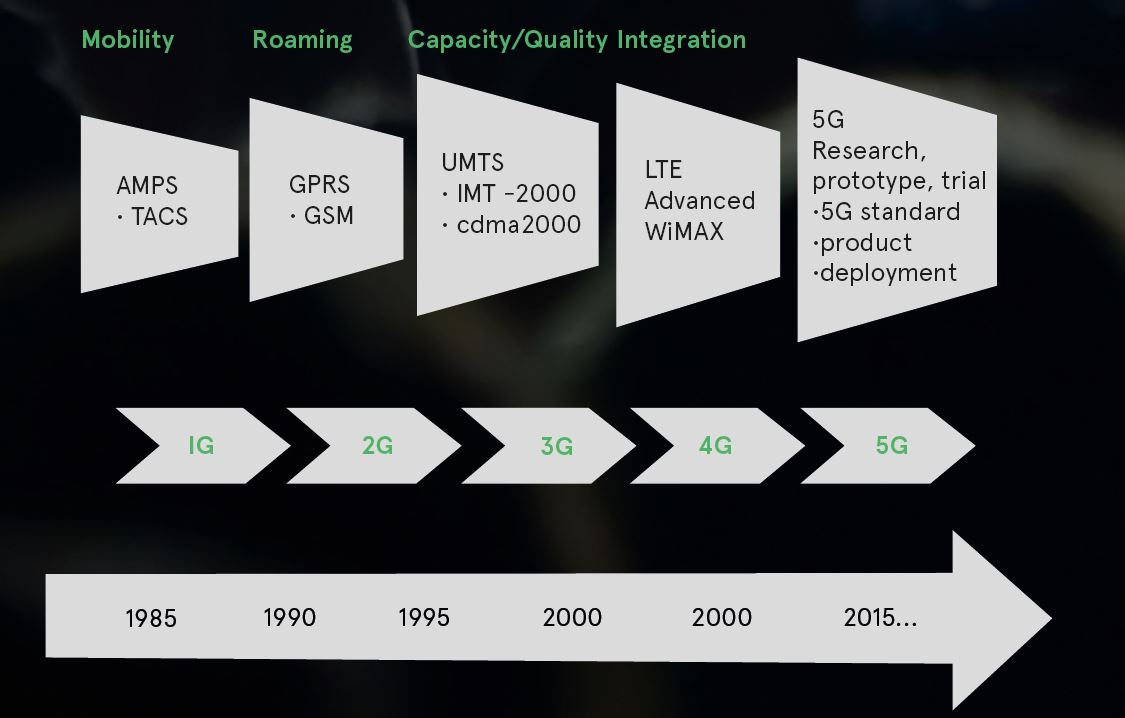
\includegraphics[width=1\linewidth]{graphics/cellular_history_timeline}
    \caption[Overzicht omtrent de geschiedenis van cellulaire netwerken]{Geschiedenis omtrent de evolutie van cellulaire netwerken \autocite{Keenan2020}}
    \label{fig:cellularhistory}
\end{figure}

\subsection{Eerste generatie}

De eerste vorm van telecommunicatie kwam er in 1979 onder de naam van 1G. Deze technologie, eerst gebruikt door de inwoners van Japan, bracht de mogelijkheid om anderen te bellen maar het had ook een groot deel aan nadelen. Zo was een gesprek niet beveiligd, was roaming geen optie en de geluidskwaliteit was laag.
De reden dat een gesprek niet beveiligd is vanwege het feit dat er geen encryptie is over het netwerk dus eender wie die wou, kon meeluisteren. Deze technologie had een trage downloadsnelheid die specifiek neerkwam op een 2.4 Kbps gemiddeld. \autocite{Galazzo2020}. Neem nu bijvoorbeeld een korte film van 10 minuten in een MP4 formaat met codec H264 en een resolutie van 1920 x 1080p met een bitrate van 10.000 kbit/s. Zo'n bestand zou 775 MB innemen. \autocite{Helme2019} Gebruik makend van de alle voorgaande informatie over dit bestand en de snelheid van netwerk is de tijd die het zou nemen om het te downloaden neerkomen op 28 dagen, 22 uur, 26 minuten en 40 seconden.

\subsection{Tweede generatie}

2G maakte zijn introductie in de wereld gedurende het jaar 1991 in Finland op de rug van het Global System voor Mobile Communications of afgekort GSM. \autocite{Galazzo2020}. Deze volgende stap definieerde een statistisch grote sprong naar verbetering ten opzichte van de eerste generatie. Men kon namelijk eindelijk berichten versturen naast bellen. Ook kon men multimedia bestanden delen zoals foto's en waren gesprekken vanaf dit punt wel geëncrypteerd en dus veilig van andermans oren. Doordat de populariteit van connectiviteit ook steeg was er ook een nood aan een efficiëntere toepassing van het spectrum zodat meer apparaten het konden gebruiken. 2G, in tegenstelling tot 1G die niet meer in wereldwijde benutting is, stelt men nog steeds in voor bepaalde toepassingen zoals het Internet of Things. \autocite{Henke2021} Indien men het voorbeeld van de kortfilm uit het eerste hoofdstuk wil herhalen nemen we de aangeboden waarde van een gemiddelde snelheid 0.2 Mbps. \autocite{Galazzo2020} Hierdoor zou de tijdsduur voor het downloaden van de kortfilm met identieke specificaties als in het eerste voorbeeld gelijkaardig zijn aan 8 uren en 20 seconden. \autocite{Wooding2024}

\subsection{Derde generatie}

De initiële inzetting van 3G kwam voor in Japan op de eerste oktober in 2001. De oorsprong hiervan ontstond uit de altijd stijgende vraag van de wereldbevolking om geconnecteerd te zijn met elkaar en verscheidene acties te kunnen uitvoeren terwijl iedereen onderweg was. Dit hield functionaliteiten in zoals videobellen, mails en video's verzenden aan de snelheid waarmee het toen mogelijk was om dit uit te voeren op een vaste computer. Om dit alles mogelijk te maken was er een nood aan hogere data snelheden en ook een beter gebruik van het spectrum om zo meer apparaten toe te laten op het netwerk. \autocite{Dulcey2020} Een technologie die hielp om dit allemaal mogelijk te maken was Code Division Multiple Access of CDMA. Dit functioneert volgens een gespreid spectrum principe. Dit zorgt ervoor dat de elektromagnetische energie tot verdeling kom op een wijdere bandbreedte dan nodig nodig is. Een voordeel van deze technologie is dat het zorgt dat het sterker beveiligd is en het helpt dat de boodschap zo goed als zeker aankomt. Een nadeel van deze technologie is dat data en geluid geen optie hebben om zich tegelijk te verdelen over het netwerk. Dit onverwacht gevolg zorgt er dus effectief voor dat als iemand aan het bellen is via CDMA er geen optie is om data binnen te halen zoals bijvoorbeeld mails. \autocite{Fendelman2021} Ten slotte om een eenvoudige vergelijking te maken met de andere cellulaire technologieën kan er een gemiddelde data transfer snelheid aannemen van 2 Mbps.\autocite{Galazzo2020} Om dit dan te vertalen naar de kortfilm bij voorgaande voorbeelden zou dit 50 minuten duren om deze data op te halen. \autocite{Wooding2024}

\subsection{Vierde generatie}

Door een nood aan hogere data snelheden werden in 2008 nieuwe standaarden gedefinieerd voor een verbeterde cellulaire technologie namelijk 4G. Men stelde als één van de doelen dat deze 1000 Mbit/s moest halen in data transfer snelheden. Een probleem waar men toen op stuitte was dat deze ambities te hoog waren gesteld. Hierdoor volgde een genoodzaakte beslissing in het tot leven roepen van LTE oftewel Long Term Evolution. Dit werd gezien als een tussenstap om zo wel een betere dienst aan te bieden tot men 4G volwaardig kon aanbieden. \autocite{Nicholls2022} Een techniek die toegepast werd in deze iteratie is Orthogonal Frequency Division Multiple Access (OFDMA). Dit werkt door subcarriers, de kleinste eenheid die data kan dragen, gegroepeerd worden in subkanalen. Men verdeelt deze eenheden dan in grotere groepen genaamd bursts die kunnen toegewezen worden aan bepaalde gebruikers. Deze manier van onderverdelen en toewijzen zorgt ervoor dat er een specifieke Quality of Service (QoS) en bandbreedte kan toegewezen worden gebaseerd op wie er verbonden is. Hierdoor word de beschikbare technologie beter ingezet dan bij vorige iteraties. \autocite{Friedmann2007} Indien men de gemiddelde 4G snelheid in Canada in 2020 neemt zoals vermeld door \textcite{Galazzo2020} namelijk 55 Mbps dan zou de eerder gebruikte theoretische data hoeveelheid 1 minuut en 50 seconden nodig hebben om over het netwerk verplaats te kunnen worden. \autocite{Wooding2024}

\subsection{Vijfde generatie}

De laatste vernieuwing op vlak van cellulaire connectiviteit kwam er in 2019 onder de naam van 5G. De noodzaak om nog een sprong te maken inzake data capaciteit, snelheid \& latentie is vanwege de opkomst van nieuwe technologieën zoals VR/AR, autonome auto's en slimme fabrieken. Deze nieuwe partijen vragen namelijk achter een geavanceerder netwerk dan voorgaand mogelijk was. Ook word er gezorgd voor een betrouwbaarder netwerk dankzij het gebruik van network slicing. Deze techniek bestaat er uit om een fysiek netwerk onder te verdelen in meerdere virtuele netwerken die dan elk een bepaalde doelgroep kunnen toegewezen krijgen. Zo kan één netwerk zorgen voor lage latentie en hoge data betrouwbaarheid wat belangrijk is voor zelf rijdende auto's ten opzichte van een ander virtueel netwerk dat zich dan eerder toespitst op hoge data volumes en hoge transfer snelheden om bijvoorbeeld een film te downloaden, waar de latentie zelf er weinig tot niet toe doet. \autocite{Flinders2024} Om een finale vergelijking te maken ten opzichte van de snelheden van andere technologieën nemen we een gemiddeld gemeten snelheid in Canada van 169.46 Mbps. \autocite{Galazzo2020} Om dit in vergelijking te stellen met voorgaande nemen we weer het fictief stuk film op en wanneer dit uitgerekend word komt dit neer op een download tijd van amper 36 seconden. \autocite{Wooding2024}

\section{Architectuur LTE netwerk}
Er kunnen 3 grote delen onderscheiden worden als er vanop een hoog niveau word neergekeken op de architectuur van deze technologie, namelijk de User Equipment oftewel UE, de Evolved UMTS Terrestrial Radio Access Network mogelijks afgekort tot E-UTRAN en ten slotte de Evolved Packet Core waarnaar verder gerefeerd zal worden als EPC. \autocite{Richard2021} Hieronder volgt een diagram die de visualisatie van het besproken netwerk afbeeld. 
\begin{figure}[!htb]
    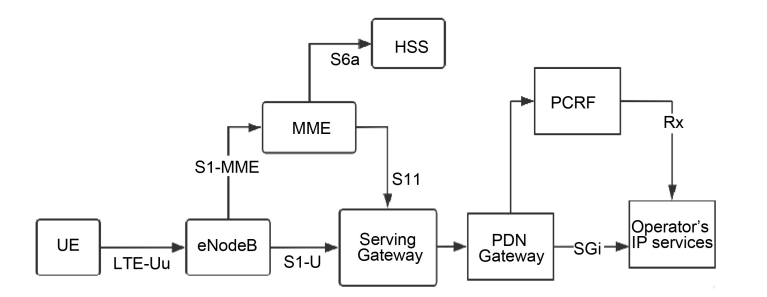
\includegraphics[width=1\linewidth]{graphics/LTE_architecture}
    \caption[Overzicht van de verscheidene componenten van de LTE architectuur.]{Diagram van verscheidene componenten en hun samenwerking binnen de LTE architectuur. \autocite{Yunman2021}}
    \label{fig:ltearchitecture}
\end{figure}

Om een uitleg te vormen omtrent E-UTRAN moet er eerst begrepen worden wat een basis Radio Access Network inhoud. Dit onderdeel kan gezien worden als het radio gedeelte om ervoor te zorgen dat eindgebruikers kunnen communiceren met de rest van het systeem. Deze kan men in de omgeving spotten als palen ook wel nodeBs genoemd die drie componenten bevatten namelijk antennes, radio's en baseband units. Elektrische pulsen omzetten naar radio signalen is het doel van de antenne. Radio's daarentegen nemen de gereguleerde energie niveaus en gereserveerde frequentie in achting zodat digitale signalen kunnen omgezet worden in objecten die men draadloos kan versturen. Ten slotte zijn er dan nog de baseband units. Om draadloze communicatie namelijk mogelijk te maken is er een nood aan functies die logisch kunnen redeneren. Deze zijn in de laatst vernoemde component te vinden. \autocite{Jones2021} \\ \\
Om dan terug te komen naar wat de E-UTRAN dan specifiek inhoud kan er een vergelijking gemaakt worden met hoe het er in de voorgaande technologieën aan toe ging. Bij deze was er namelijk een nodeB zoals bij voorgaande besproken maar belangrijk is dat er hierbij ook een controller aanwezig is. De voornaamste taken van dit object waren het beheren van beschikbare middelen en het bijhouden van de verplaatsingen van een bepaalde eindgebruiker om zo deze door te kunnen geven van de ene nodeB naar de andere. Bij deze geëvolueerde versie daarvan valt de controller weg en smelt deze samen met de node zorgende voor een eNode. \autocite{Ghayas2019} Het feit dat alle functionaliteit verwoven zit in de node zelf zorgt voor lagere latency doordat er een hechte samenwerking is tussen de verschillende protocol lagen. Ook elimineert het een single point of failure en verlaagt het de kost. \autocite{Palat2011} \\

Nadat een UE verbonden is met een eNodeB word de data doorgestuurd naar de EPC. Dit systeem is een framework die verschillende functionaliteiten ondersteunt. Het verschil met voorgaande technologieën is dat het IP services zijn in plaats van circuit of packet switching. \autocite{Awati2024} Maar alvorens er kan gekeken worden naar wat dit verschil inhoud moet men eerst verstaan waar de twee voorgaande technologieën voor staan. Om te beginnen met circuit switching, dit vanwege het feit dat deze de originele manier was van connecteren bij de eerste telefonie. Deze technologie bestaat eruit om eerst een verbinding op te stellen tussen bron en doel om dan hier data op te verzenden. Deze gebruikers krijgen dan elk een bepaald toegewezen deel van de bandbreedte, wat er voor zorgt dat wanneer men niets verzend de ruimte wel word vrijgehouden wat zorgt voor ferme verspilling. Door de groei in aantal eindgebruikers die het netwerk gebruikten werd de noodzaak groter om over te schakelen van een circuit naar de volgende iteratie namelijk een packet switched netwerk. Hierbij is het de bedoeling om data te verpakken in pakketten bestaande uit een header en de effectieve data. Dit eerste deel zorgt ervoor dat wanneer de data toekomt bij de ontvanger deze ze mogelijk nog kan herorganiseren wanneer ze in een andere volgorde zouden toekomen. Hierdoor hebben ze een netwerk enkel nodig gedurende de tijd dat het pakket onderweg is, wat zorgt dat het veel eerder vrij is voor anderen dan bij de voorgaande technologie. \autocite{BasuMallick2022} Bij IP services is het dan de bedoeling om stem en data te versturen op basis van IP-pakketten die verzonden worden van de ene gebruiker met een toegewezen ip adres en de andere met ook zo'n adres dat ze toegewezen kregen op het moment dat ze voor het eerst verbonden met de cel. Deze verandering zorgt ervoor dat het de netwerken versimpelt terwijl het netwerk hoge performantie en capaciteit behoud. \autocite{Awati2024} \\

Een eerste onderdeel van het EPC is de Mobility Management Entity oftewel MME. Deze procedure is verantwoordelijk voor de authenticatie, autorisatie en de locatie van een eindgebruiker bij te houden. Dit stuk is ook rechtstreeks verbonden met de eNodeBs. Deze groep van base stations is dan weer onderverdeeld in kleinere groepen van Tracking Areas. Deze TA's kan men dan oplijsten in groeperingen van TA's die dicht bij elkaar liggen. Deze TAL is belangrijk vanwege het feit dat de MME bijhoud welke TAL's er waar mogelijk zijn en dat een UE ook uitzend naar buiten met welke TAL ze huidig verbonden zijn. Wanneer de UE dan buiten zijn TAL loopt dan start het een procedure met de MME om een nieuwe TAL toegewezen word. Naast deze info houd de MME ook de laatst verbonden cel bij, dit zodat wanneer men bijvoorbeeld iemand probeert te bellen de MME eerst de laatst verbonden cel contacteert om te zien of de UE kan bereikt worden, indien dit niet lukt vergroten ze hun zoektocht naar de volledige TAL om toch de UE te kunnen bereiken. \autocite{Liou2013} \\

De MME is een onderdeel van het controle gedeelte van de architectuur maar er is ook een niveau dat omgaat met de data te behandelen die de gebruiker wil ophalen of versturen. Een van de componenten die daarvoor instaat is de SGW oftewel Serving Gateway. Dit onderdeel staat in contact met de MME en zorgt voor het doorgeven van data maar ook het verzorgen van de Quality of Service doorheen het data vlak. Men verbind een MME met de SGW omdat wanneer een gebruiker zich voor het eerst registreert bij een netwerk de registratie voltrokken word bij de MME maar deze hierna een signaal moet geven aan de andere componenten om de data stroom ook wel degelijk te starten. Vandaar dat er een link is tussen deze twee elementen. \autocite{Malla2014} \\

Het controle gedeelte van een LTE architectuur bestaat wel niet enkel uit een MME maar bevat ook een Home Subscriber Server (HSS). Deze service bestaat er uit om te fungeren als een databank waarin alle relevante data zich herbergt omtrent de gebruikers. Deze data kan info bevatten dat te maken heeft met locatie, quality of service niveau en roaming rechten indien de gebruiker geen subscriptie heeft bij het huidig netwerk waar het op is aangesloten. Deze component staat rechtstreeks in contact met de MME zodat deze de huidige data kan uitlezen of aanpassen om zo concrete acties uit te kunnen voeren gedurende dat een eindgebruiker verbonden is met het netwerk. \autocite{Shinde2020} \\

Het laatste onderdeel van het data niveau dat tussen de eindgebruiker en het data netwerk zelf staat is de Packet Data Network Gateway (PDN GW). Dit onderdeel krijgt alle data door van de SGW. Dit punt zorgt in principe voor een mogelijkheid om zowel 3GPP, zoals 5G, 4G etc., en niet-3GPP technologieën, zoals WiMax en CDMA 1x of EvDO,  te gebruiken wanneer men wil verbinden met anderen. Een andere functionaliteit waar deze service voor instaat is het filteren van bepaalde pakketten op een gebruikers niveau. Dit doet men door een diepere inspectie te doen op de pakketten die de revue passeren. Doordat men zo'n diepe inspectie doet op wat en wanneer er passeert kan men ook vanuit het gerecht delen onderscheppen en meeluisteren. \autocite{Gilbert2012}      

\section{Data terminologie}

Vooraleer men bepaalde maatstaven bespreekt omtrent de kwaliteit van een specifiek signaal tussen zendmast en eindgebruiker is het belangrijk om een uitleg te geven bij de verschillende meeteenheden die vaak gebruikt worden omtrent deze situaties. Eerst en vooral is er een decibel of dB. In de omgeving van een radio signalen staat deze meeteenheid voor het ratio van verlies of winst dat een bepaald apparaat genereert op een specifiek signaal. Zo kan een kabel voor x dB verlies zorgen van het signaal. Belangrijk bij deze meeteenheid is ook dat de schaal hiervan niet lineair is maar logaritmisch. Wat betekend dat indien een bepaald apparaat de kracht van een signaal halveert, de dB waarde die hieraan gelinkt gaat stijgt of daalt met een stap van 3. Dus neem nu bijvoorbeeld een signaal die door een kabel gaat waar er 9dB verlies op staat, dan betekend dit dat het 3 maal gehalveerd word in kracht alvorens het de kabel verlaat. \autocite{Young2004} \\

Naast een dB waarde dat vooral een ratio is voor hoeveel winst/verlies er zit op een bepaald element is het belangrijk om deze waarde ook te staven ten opzichte van andere standaarden om hieruit verdere bruikbare waarden uit op te halen. Zo kan men het aantal decibel per milliwatt staven onder de naam dBm. Wat dat dus betekent is dat deze maateenheid meet met hoeveel kracht een bepaald signaal word uitgezonden. Hoe lager deze waarde, hoe slechter je signaal. Wel moet men opletten dat wanneer deze waarde te hoog is er een mogelijkheid is dat de kracht van dit signaal er voor zorgt dat ruis en interferentie ook groter worden dat wederom ook zorgt voor een slechter signaal. \autocite{Hardesty2023} \\

Een waarde die vaak voorkomt wanneer men de kwaliteit en sterkte van een netwerk meet is RSSI oftewel Received Signal Strength Indicator. Van al de komende schalen en meetstaven is deze de basis. De numerieke waarde die men hieruit terugkrijgt is namelijk een bepaald punt op een schaal gaande van 0, perfecte verbinding, tot -100, wat staat voor helemaal geen bereik. Wanneer dit gemeten word neemt het veel factoren op in de berekening maar het is niet perfect vanwege het feit dat het geen rekening houd met ruis, onderbrekingen van andere bronnen of hoe betrouwbaar de verbinding wel is.  \autocite{Ramirez2023} \\

Een andere waarde die kan opgemeten wanneer men verbonden is met een bepaalde cel is de RSRP of Reference Signal Received Power. Dit definieêrt namelijk hoe goed en standvast de verbinding tussen een eindgebruiker en de huidige mast is. De schaal die deze parameter gebruikt is gelijkaardig aan die van RSSI, namelijk dat het negatieve waarden zijn en lager wijst op een slechtere verbinding maar de schaal loopt van -50 tot -130 dBm. De factor die voor een grote impact hierop zorgt is de afstand tot aan de effectieve mast en of de eindgebruiker een duidelijke zichtlijn zonder obstakels heeft met hiervoor vermelde toren. \autocite{Ramirez2023} \\

Gebruik makende van de vorige twee waarden kan men een andere waarde berekenen die meer inzicht geeft in hoe efficiënt het netwerk data oplevert en of er een betrouwbare connectie is. \autocite{Apostu2024} Deze waarde word ook wel RSRQ oftewel Reference Signal Received Quality genoemd en kan berekend worden met een van de volgende formules:

$ RSRP (Watt) = N \times RSRP / RSSQ $ \\
$ RSRP (dBm) = log_{10} (N) + RSRP - RSSI $

In beide van deze is er een nood voor een waarde N waarmee hier gerefereerd wordt naar het nummer van resource blocks aanwezig in de gemeten bandbreedte van de cel waarmee men verbonden is. \autocite{Kovadloff2021} Deze componenten zijn groeperingen van 12 sub carriers wat uiteindelijk uitkomt op een blok van 180 kHz. \autocite{Mishra2018} Op onderstaande figuur kan men zien hoe het aantal beschikbare blokken zich verhoudt tot de verschillende bandbreedtes die momenteel aanwezig zijn op de markt. 

\begin{figure*}[ht]
    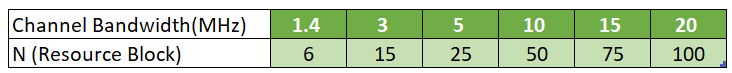
\includegraphics[width=1\linewidth]{graphics/bandwithandRB}
    \caption[Relatie tussen bandbreedte en resource blocks]{Relatie tussen bandbreedte en resource blocks \autocite{Kovadloff2021}}
    \label{fig:bandwithandrb}
\end{figure*}

Wanneer men wil bepalen in welke capaciteit een bepaald bericht kan getransporteerd worden over een netwerk is het belangrijk om de ruis aanwezig ook in te calculeren. Een maat staaf die daarvoor kan ingezet worden is Signal to Noise Ratio (SNR). Dit geeft een ratio weer van de signaal sterkte ten opzichte van de ruis aanwezig. Deze waarde word zoals de voorgaande weergegeven in dBm. Afgaande van hoe het ratio is opgesteld is ook duidelijk dat hoe dichter deze waarde nadert bij de nul, hoe slechter het netwerk er aan toe is en er een lagere kans is dat een bepaald object ook effectief kan verstuurd worden.  \autocite{Sheldon2021}

\section{Commercieel alternatief}

Om de kwaliteit van een proof-of-concept vast te stellen zal deze vergeleken worden met een alternatief dat al reeds op de markt is en waarvan deze in gebruik is door de doelgroep. Na nader onderzoek blijkt dit G-NetTrack Pro te zijn die in gebruik is door Citymesh. Deze applicatie werd ontwikkeld door Gyokov Solutions om informatie omtrent een netwerk te kunnen verzamelen. Deze data is dan inzetbaar in andere applicaties binnen hun ecosysteem om zo analyses en dergelijke te nemen.\autocite{Solutions2024}  Aanwezige functionaliteiten bevatten maar beperken zich niet tot:

\begin{itemize}
    \item Informatie van een cel verkrijgen, alsook de daar rond liggende cellen
    \item Accurate metingen binnen en buiten.
    \item Ondersteuning voor apparaten die gebruik maken van dual SIM technologie.
    \item Andere manieren om data te representeren zoals een kaart
\end{itemize}

% Dit hoofdstuk bevat je literatuurstudie. De inhoud gaat verder op de inleiding, maar zal het onderwerp van de bachelorproef *diepgaand* uitspitten. De bedoeling is dat de lezer na lezing van dit hoofdstuk helemaal op de hoogte is van de huidige stand van zaken (state-of-the-art) in het onderzoeksdomein. Iemand die niet vertrouwd is met het onderwerp, weet nu voldoende om de rest van het verhaal te kunnen volgen, zonder dat die er nog andere informatie moet over opzoeken \autocite{Pollefliet2011}.

% Je verwijst bij elke bewering die je doet, vakterm die je introduceert, enz.\ naar je bronnen. In \LaTeX{} kan dat met het commando \texttt{$\backslash${textcite\{\}}} of \texttt{$\backslash${autocite\{\}}}. Als argument van het commando geef je de ``sleutel'' van een ``record'' in een bibliografische databank in het Bib\LaTeX{}-formaat (een tekstbestand). Als je expliciet naar de auteur verwijst in de zin (narratieve referentie), gebruik je \texttt{$\backslash${}textcite\{\}}. Soms is de auteursnaam niet expliciet een onderdeel van de zin, dan gebruik je \texttt{$\backslash${}autocite\{\}} (referentie tussen haakjes). Dit gebruik je bv.~bij een citaat, of om in het bijschrift van een overgenomen afbeelding, broncode, tabel, enz. te verwijzen naar de bron. In de volgende paragraaf een voorbeeld van elk.

% \textcite{Knuth1998} schreef een van de standaardwerken over sorteer- en zoekalgoritmen. Experten zijn het erover eens dat cloud computing een interessante opportuniteit vormen, zowel voor gebruikers als voor dienstverleners op vlak van informatietechnologie~\autocite{Creeger2009}.

% Let er ook op: het \texttt{cite}-commando voor de punt, dus binnen de zin. Je verwijst meteen naar een bron in de eerste zin die erop gebaseerd is, dus niet pas op het einde van een paragraaf.

%%=============================================================================
%% Methodologie
%%=============================================================================

\chapter{\IfLanguageName{dutch}{Methodologie}{Methodology}}%
\label{ch:methodologie}

%% TODO: In dit hoofstuk geef je een korte toelichting over hoe je te werk bent
%% gegaan. Verdeel je onderzoek in grote fasen, en licht in elke fase toe wat
%% de doelstelling was, welke deliverables daar uit gekomen zijn, en welke
%% onderzoeksmethoden je daarbij toegepast hebt. Verantwoord waarom je
%% op deze manier te werk gegaan bent.
%% 
%% Voorbeelden van zulke fasen zijn: literatuurstudie, opstellen van een
%% requirements-analyse, opstellen long-list (bij vergelijkende studie),
%% selectie van geschikte tools (bij vergelijkende studie, "short-list"),
%% opzetten testopstelling/PoC, uitvoeren testen en verzamelen
%% van resultaten, analyse van resultaten, ...
%%
%% !!!!! LET OP !!!!!
%%
%% Het is uitdrukkelijk NIET de bedoeling dat je het grootste deel van de corpus
%% van je bachelorproef in dit hoofstuk verwerkt! Dit hoofdstuk is eerder een
%% kort overzicht van je plan van aanpak.
%%
%% Maak voor elke fase (behalve het literatuuronderzoek) een NIEUW HOOFDSTUK aan
%% en geef het een gepaste titel.

Gedurende de eerste fase van het onderzoek zal een literatuurstudie opgesteld worden. Deze is terug te vinden in hoofdstuk 2 onder de stand van zaken en bespreekt onderwerpen gaande van de geschiedenis omtrent telecommunicatie netwerken tot de structuur van een LTE netwerk en zelfs een diepgaande uitleg omtrent verschillende termen die vaak voorkomend zijn wanneer men de kwaliteit van een bepaald signaal bespreekt. \\

De tweede fase bestaat er uit om een requirement analyse uit te voeren zodat er een beeld kan gevormd worden aan wat de applicatie dient te voldoen om effectief ingezet te kunnen worden in het werkveld om zo functioneel netwerken te testen. De voorwaarden die bij deze stap neergezet worden kan men dan nadien ook inzetten om de nieuwe applicatie te vergelijken met andere applicaties die al reeds op de markt zijn, of in gebruik zijn binnen Citymesh. Dit onderdeel zal hieronder in een apart hoofdstuk besproken worden. \\

Doorheen de derde fase zal er dan een Proof-of-Concept opgesteld worden gebaseerd op de eerder gestelde voorwaarden. Dit zal gebeuren in meerdere iteraties en met terugkoppeling naar de poule van eindgebruikers voor de te ontwikkelen tool. \\

Ten slotte worden de oude en nieuwe tool tegenover elkaar gezet in een labo omgeving waarin testen zullen uitgevoerd worden om zo te zien of er significante voordelen zijn geboekt bij het opbouwen van de nieuwe applicatie ten opzichte van de reeds bestaande technologie. Hierover zal dan een conclusie gevormd worden met advies richting Citymesh zodat men gebruik makende van de beste tool verder hun netwerken kan testen.

\section{Requirementsanalyse}

Om een grondig antwoord te formuleren op de gestelde vraag is het noodzakelijk om vast te leggen wat er van een bepaalde applicatie met dit doel verwacht word. Om deze functionaliteiten een bepaalde prioriteit toe te kennen zal gebruik gemaakt worden van de MoScoW-methode. Hierbij zal elke nood onderverdeeld een plaats krijgen in een bepaalde categorie. Eest en vooral is er de 'Must have', dit bestaat uit de functionaliteiten die een tool moet hebben of deze kan niet gerekend worden als een mogelijke oplossing voor het probleem. Een trap lager is er dan de 'Should have', dit representeert het deel dat belangrijk is, maar niet essentieel. Ten derde is er dan de 'Could have' categorie, dit is dan de groep van functionaliteiten met een lage prioriteit maar waarvan het bestaan wel goed is voor het product. Ten slotte is er ook nog de 'Won't have' functionaliteiten. Hieronder verstaat men de prioriteiten waaraan geen aandacht moet besteed worden vanwege het feit dat dit een lage prioriteit heeft of het niet nodig is in de huidige iteratie richting een product. \autocite{Khan2015}



% Voeg hier je eigen hoofdstukken toe die de ``corpus'' van je bachelorproef
% vormen. De structuur en titels hangen af van je eigen onderzoek. Je kan bv.
% elke fase in je onderzoek in een apart hoofdstuk bespreken.

%\input{...}
%\input{...}
%...

%%=============================================================================
%% Conclusie
%%=============================================================================

\chapter{Conclusie}%
\label{ch:conclusie}

% TODO: Trek een duidelijke conclusie, in de vorm van een antwoord op de
% onderzoeksvra(a)g(en). Wat was jouw bijdrage aan het onderzoeksdomein en
% hoe biedt dit meerwaarde aan het vakgebied/doelgroep? 
% Reflecteer kritisch over het resultaat. In Engelse teksten wordt deze sectie
% ``Discussion'' genoemd. Had je deze uitkomst verwacht? Zijn er zaken die nog
% niet duidelijk zijn?
% Heeft het onderzoek geleid tot nieuwe vragen die uitnodigen tot verder 
%onderzoek?

Dit onderzoek stemt voort uit volgende onderzoeksvraag:
\begin{itemize}
    \item Hoe kan het ontwikkelen van een interne applicatie het handmatig testen van een privaat netwerk vereenvoudigen?
\end{itemize}

Na een grondige literatuurstudie en een daaropvolgend praktisch onderzoek is het mogelijk om hierop een antwoord te formuleren. De verkregen Proof of Concept en het gebruik hiervan legt namelijk duidelijke pijn- en pluspunten te boven. Deze applicatie werd ontwikkeld om het proces omtrent de testen toegepast op een netwerk te stroomlijnen. Voor de arbeidsintensieve taak omtrent het veld zelf afgaan is dit namelijk niet mogelijk. Een persoon die  een bepaalde tour rond het terrein loopt zal altijd noodzakelijk blijven. Wel kon er opgemaakt worden dat de data die verzameld werd door de POC adequaat van niveau was ten opzichte van het commercieel alternatief. De data verwerken die voortkwam uit beide applicaties bleek wel minder tijd consumerend bij de POC. Dit vanwege het feit dat deze werd bijgehouden in een externe database ten opzichte van een data dump in de vorm van een .txt bestand op het apparaat zelf bij de andere applicatie. Nadien is er dus minder werk om tot conclusies te komen gebruikmakende van de aanwezige data. Er was in de POC ook meer flexibiliteit aanwezig omtrent de soorten testen die men kon uitvoeren. Zo was het mogelijk om een speciale routine te voorzien gebaseerd op een specifieke situatie i.p.v. de één soort test die de andere applicatie aanbood.\\

Uit dit onderzoek kunnen wel andere onderzoeksvragen geformuleerd worden namelijk:
\begin{itemize}
    \item In welke capaciteit heeft het direct verzenden van data een invloed op het netwerk dat men test?
    \item Kan een applicatie testen op de achtergrond uitvoeren en resulteert dit in gelijkaardige resultaten ten opzichte van testen uitgevoerd op de voorgrond?
\end{itemize}



%---------- Bijlagen -----------------------------------------------------------

\appendix

\chapter{Onderzoeksvoorstel}

Het onderwerp van deze bachelorproef is gebaseerd op een onderzoeksvoorstel dat vooraf werd beoordeeld door de promotor. Dat voorstel is opgenomen in deze bijlage.

%% TODO: 
%\section*{Samenvatting}

% Kopieer en plak hier de samenvatting (abstract) van je onderzoeksvoorstel.

% Verwijzing naar het bestand met de inhoud van het onderzoeksvoorstel
%---------- Inleiding ---------------------------------------------------------

\section{Introductie}%
\label{sec:introductie}

\subsection{Kaderen thema}

\subsection{De doelgroep}

\subsection{Probleemstelling en onderzoeksvraag}

\subsection{De onderzoeksdoelstelling}

Waarover zal je bachelorproef gaan? Introduceer het thema en zorg dat volgende zaken zeker duidelijk aanwezig zijn:

\begin{itemize}
  \item kaderen thema
  \item de doelgroep
  \item de probleemstelling en (centrale) onderzoeksvraag
  \item de onderzoeksdoelstelling
\end{itemize}

Denk er aan: een typische bachelorproef is \textit{toegepast onderzoek}, wat betekent dat je start vanuit een concrete probleemsituatie in bedrijfscontext, een \textbf{casus}. Het is belangrijk om je onderwerp goed af te bakenen: je gaat voor die \textit{ene specifieke probleemsituatie} op zoek naar een goede oplossing, op basis van de huidige kennis in het vakgebied.

De doelgroep moet ook concreet en duidelijk zijn, dus geen algemene of vaag gedefinieerde groepen zoals \emph{bedrijven}, \emph{developers}, \emph{Vlamingen}, enz. Je richt je in elk geval op it-professionals, een bachelorproef is geen populariserende tekst. Eén specifiek bedrijf (die te maken hebben met een concrete probleemsituatie) is dus beter dan \emph{bedrijven} in het algemeen.

Formuleer duidelijk de onderzoeksvraag! De begeleiders lezen nog steeds te veel voorstellen waarin we geen onderzoeksvraag terugvinden.

Schrijf ook iets over de doelstelling. Wat zie je als het concrete eindresultaat van je onderzoek, naast de uitgeschreven scriptie? Is het een proof-of-concept, een rapport met aanbevelingen, \ldots Met welk eindresultaat kan je je bachelorproef als een succes beschouwen?

%---------- Stand van zaken ---------------------------------------------------

\section{State-of-the-art}%
\label{sec:state-of-the-art}

Hier beschrijf je de \emph{state-of-the-art} rondom je gekozen onderzoeksdomein, d.w.z.\ een inleidende, doorlopende tekst over het onderzoeksdomein van je bachelorproef. Je steunt daarbij heel sterk op de professionele \emph{vakliteratuur}, en niet zozeer op populariserende teksten voor een breed publiek. Wat is de huidige stand van zaken in dit domein, en wat zijn nog eventuele open vragen (die misschien de aanleiding waren tot je onderzoeksvraag!)?

Je mag de titel van deze sectie ook aanpassen (literatuurstudie, stand van zaken, enz.). Zijn er al gelijkaardige onderzoeken gevoerd? Wat concluderen ze? Wat is het verschil met jouw onderzoek?

Verwijs bij elke introductie van een term of bewering over het domein naar de vakliteratuur, bijvoorbeeld~\autocite{Hykes2013}! Denk zeker goed na welke werken je refereert en waarom.

Draag zorg voor correcte literatuurverwijzingen! Een bronvermelding hoort thuis \emph{binnen} de zin waar je je op die bron baseert, dus niet er buiten! Maak meteen een verwijzing als je gebruik maakt van een bron. Doe dit dus \emph{niet} aan het einde van een lange paragraaf. Baseer nooit teveel aansluitende tekst op eenzelfde bron.

Als je informatie over bronnen verzamelt in JabRef, zorg er dan voor dat alle nodige info aanwezig is om de bron terug te vinden (zoals uitvoerig besproken in de lessen Research Methods).

% Voor literatuurverwijzingen zijn er twee belangrijke commando's:
% \autocite{KEY} => (Auteur, jaartal) Gebruik dit als de naam van de auteur
%   geen onderdeel is van de zin.
% \textcite{KEY} => Auteur (jaartal)  Gebruik dit als de auteursnaam wel een
%   functie heeft in de zin (bv. ``Uit onderzoek door Doll & Hill (1954) bleek
%   ...'')

Je mag deze sectie nog verder onderverdelen in subsecties als dit de structuur van de tekst kan verduidelijken.

%---------- Methodologie ------------------------------------------------------
\section{Methodologie}%
\label{sec:methodologie}

Hier beschrijf je hoe je van plan bent het onderzoek te voeren. Welke onderzoekstechniek ga je toepassen om elk van je onderzoeksvragen te beantwoorden? Gebruik je hiervoor literatuurstudie, interviews met belanghebbenden (bv.~voor requirements-analyse), experimenten, simulaties, vergelijkende studie, risico-analyse, PoC, \ldots?

Valt je onderwerp onder één van de typische soorten bachelorproeven die besproken zijn in de lessen Research Methods (bv.\ vergelijkende studie of risico-analyse)? Zorg er dan ook voor dat we duidelijk de verschillende stappen terug vinden die we verwachten in dit soort onderzoek!

Vermijd onderzoekstechnieken die geen objectieve, meetbare resultaten kunnen opleveren. Enquêtes, bijvoorbeeld, zijn voor een bachelorproef informatica meestal \textbf{niet geschikt}. De antwoorden zijn eerder meningen dan feiten en in de praktijk blijkt het ook bijzonder moeilijk om voldoende respondenten te vinden. Studenten die een enquête willen voeren, hebben meestal ook geen goede definitie van de populatie, waardoor ook niet kan aangetoond worden dat eventuele resultaten representatief zijn.

Uit dit onderdeel moet duidelijk naar voor komen dat je bachelorproef ook technisch voldoen\-de diepgang zal bevatten. Het zou niet kloppen als een bachelorproef informatica ook door bv.\ een student marketing zou kunnen uitgevoerd worden.

Je beschrijft ook al welke tools (hardware, software, diensten, \ldots) je denkt hiervoor te gebruiken of te ontwikkelen.

Probeer ook een tijdschatting te maken. Hoe lang zal je met elke fase van je onderzoek bezig zijn en wat zijn de concrete \emph{deliverables} in elke fase?

%---------- Verwachte resultaten ----------------------------------------------
\section{Verwacht resultaat, conclusie}%
\label{sec:verwachte_resultaten}

Hier beschrijf je welke resultaten je verwacht. Als je metingen en simulaties uitvoert, kan je hier al mock-ups maken van de grafieken samen met de verwachte conclusies. Benoem zeker al je assen en de onderdelen van de grafiek die je gaat gebruiken. Dit zorgt ervoor dat je concreet weet welk soort data je moet verzamelen en hoe je die moet meten.

Wat heeft de doelgroep van je onderzoek aan het resultaat? Op welke manier zorgt jouw bachelorproef voor een meerwaarde?

Hier beschrijf je wat je verwacht uit je onderzoek, met de motivatie waarom. Het is \textbf{niet} erg indien uit je onderzoek andere resultaten en conclusies vloeien dan dat je hier beschrijft: het is dan juist interessant om te onderzoeken waarom jouw hypothesen niet overeenkomen met de resultaten.



%%---------- Andere bijlagen --------------------------------------------------
% TODO: Voeg hier eventuele andere bijlagen toe. Bv. als je deze BP voor de
% tweede keer indient, een overzicht van de verbeteringen t.o.v. het origineel.
%\input{...}

%%---------- Backmatter, referentielijst ---------------------------------------

\backmatter{}

\setlength\bibitemsep{2pt} %% Add Some space between the bibliograpy entries
\printbibliography[heading=bibintoc]

\end{document}
